% Copyright (c) 2023 Zachary Todd Edwards
% MIT License

% Must be compiled with lualatex and -shell-escape
% gnuplot required
\documentclass[12pt]{article}
\usepackage{savetrees}
\usepackage{parskip}

\usepackage{fontspec}
\setmainfont{ubuntu}[
    Path        =   ../common/fonts/,
    Extension   =   .ttf,
    UprightFont =   *-R,
    BoldFont    =   *-B,
]
\setmonofont{ubuntumono}[
  Path          =   ../common/fonts/,
  Extension     =   .ttf,
  UprightFont   =   *-R,
  BoldFont      =   *-B,
  ItalicFont    =   *-RI,
]

% Copyright (c) 2023 Zachary Todd Edwards
% MIT License

\usepackage{pgfplots}
\pgfplotsset{compat=1.17}
\usepackage{adjustbox}
\usepackage{float}
\usepackage{caption}

\usepackage{xcolor}
\definecolor{codegray}{RGB}{128,128,128}
\definecolor{line_color}{RGB}{0,51,160}
\definecolor{mark_color}{RGB}{177,2,2}
\definecolor{avg_color}{RGB}{255, 163, 0}

\usepackage{listings}
\lstset{
  language=C++, % choose the language of the code
  basicstyle=\ttfamily\footnotesize,
  numberstyle=\tiny\color{codegray},
  numbers=left, % where to put the line-numbers
  numbersep=5pt,
}

%For getting the average of a parametric equation using gnuplot
\usepackage{shellesc}

\newcounter{PolynomialID}
\newcommand\getPolynomialID{polynomial\thePolynomialID}
\newcommand{\polynomial}[3][0.9\columnwidth]{
  \begin{figure}[H]
    \begin{center}
      \begin{adjustbox}{width = #1}
        \begin{tikzpicture}
          \begin{axis}[
              axis lines=center,
              xmin=-6, xmax=6,
              ymin=-6, ymax=6,
              xtick={-5,-4,...,5},
              ytick={-5,-4,...,5},
              domain = -6:6,
              restrict y to domain=-20:20,
              xtick distance=1,
              ytick distance=1,
              grid=major,
              grid style = {solid},
              yticklabels={,,},
              xticklabels={,,},]
            \addplot[id=\getPolynomialID,samples=100,line_color,style={thick},smooth] {#2};
          \end{axis}
        \end{tikzpicture}
      \end{adjustbox}
    \end{center}
    \caption*{#3}
  \end{figure}
  \stepcounter{PolynomialID}
}

\newcounter{MarkID}
\newcommand\getMarkID{mark\theMarkID}

\newcounter{WaveID}
\newcommand\getWaveID{wave\theWaveID}
\newlength{\wavewidth}
\newcommand{\waveform}[4][0.9\columnwidth]{% args: size, function(x), marks, caption
  \setlength{\wavewidth}{#1}
  \begin{figure}[H]
    \begin{center}
      \begin{tikzpicture}
        \begin{axis}[
            axis lines=center,
            tick pos = right,
            width = \wavewidth,
            height = 0.19\wavewidth,
            xmin=0, xmax=4,
            ymin=-2, ymax=2,
            xtick={1,2,3},
            ytick={-1,0,1},
            domain = 0:4,
            restrict y to domain=-4:4,
            xtick distance=1,
            ytick distance=1,
            grid=major,
            grid style = {solid},
            yticklabels={,,},
            xticklabels={,,},]
          \addplot[id=\getWaveID,samples=400,line_color,style={thick},smooth] function{#2};
          \ifnum#3>0
            \addplot[id=\getMarkID,samples=#3,mark_color,only marks, mark=*] function{#2};
            \stepcounter{MarkID}
          \fi
        \end{axis}
      \end{tikzpicture}
    \end{center}
    \caption*{#4}
  \end{figure}
  \stepcounter{WaveID}
}

\newcommand{\criticalFrequency}[2][0.9\columnwidth]{% args: size, caption
  \setlength{\wavewidth}{#1}
  \begin{figure}[H]
    \begin{center}
      \begin{tikzpicture}
        \begin{axis}[
            axis lines=center,
            tick pos = right,
            width = \wavewidth,
            height = 0.19\wavewidth,
            xmin=0, xmax=4,
            ymin=-2, ymax=2,
            xtick={1,2,3},
            ytick={-1,0,1},
            domain = 0:4,
            restrict y to domain=-4:4,
            xtick distance=1,
            ytick distance=1,
            grid=major,
            grid style = {solid},
            yticklabels={,,},
            xticklabels={,,},]
          \addplot[id=\getWaveID,samples=400,line_color,style={thick},smooth] function{cos(2*2*pi*x + 0.5) - sin(2*2*pi*x) * tan(0.5)};
          \stepcounter{WaveID}
          \addplot[id=\getWaveID,samples=400,mark_color,style={thick},smooth] function{cos(2*2*pi*x + 0.8) - sin(2*2*pi*x) * tan(0.8)};
          \stepcounter{WaveID}
          \addplot[id=\getWaveID,samples=400,avg_color,style={thick},smooth] function{cos(2*2*pi*x + 0.2) - sin(2*2*pi*x) * tan(0.2)};
          \stepcounter{WaveID}
          \addplot[only marks, black, mark=*] coordinates
            {(0.23,-1.1) (0.48,1.1)
              (0.73,-1.1) (0.98,1.1)
              (1.23,-1.1) (1.48,1.1)
              (1.73,-1.1) (1.98,1.1)
              (2.23,-1.1) (2.48,1.1)
              (2.73,-1.1) (2.98,1.1)
              (3.23,-1.1) (3.48,1.1)
              (3.73,-1.1) (3.98,1.1)};
        \end{axis}
      \end{tikzpicture}
    \end{center}
    \caption*{#2}
  \end{figure}
}

\newcounter{PhasorID}
\newcommand\getPhasorID{phasor\thePhasorID}
\newcommand\genPhasorTableFilename{\jobname.\getPhasorID.table}

\newcommand{\calcPhasorAverage}[1][\genPhasorTableFilename]{% arg: filename
  \ShellEscape{gnuplot -e "stats '#1' using 1; x_avg = STATS_mean; stats '#1' using 2; y_avg = STATS_mean; set print '#1.avg'; print x_avg, y_avg"}%
}

% args: size, equation(t), period, marks, caption
% mark being 0 turns off the average indicator, 1 only average indicator, > 1 marks & average
\newcommand{\phasor}[5][0.9\columnwidth]{
  \begin{figure}[H]
    \begin{center}
      \begin{adjustbox}{width = #1}
        \begin{tikzpicture}
          \begin{axis}[
              axis lines=center,
              xmin=-4, xmax=4,
              ymin=-4, ymax=4,
              xtick={-3,-2,...,3},
              ytick={-3,-2,...,3},
              xlabel={$\Re$},
              ylabel={$\Im$},
              xtick distance=1,
              ytick distance=1,
              grid=major,
              grid style = {solid},
              yticklabels={,,},
              xticklabels={,,},]
            \addplot gnuplot[parametric,id=\getPhasorID,domain=0:8,samples=1000,line_color,style={thick},smooth,solid, no markers] {
                (#2) * cos((-2 * pi * t) * (#3)),
                (#2) * sin((-2 * pi * t) * (#3))
              };
            \ifnum#4>1
              \addplot gnuplot[parametric,id=\getMarkID,domain=0:4,samples=#4,mark_color,only marks, mark=*] {
                  (#2) * cos((-2 * pi * t) * (#3)),
                  (#2) * sin((-2 * pi * t) * (#3))
                };
              \stepcounter{MarkID}
            \fi
            \ifnum#4>0
              \calcPhasorAverage
              \addplot[mark=*,avg_color] table {\genPhasorTableFilename.avg};
            \fi
          \end{axis}
        \end{tikzpicture}
      \end{adjustbox}
    \end{center}
    \caption*{#5}
  \end{figure}
  \stepcounter{PhasorID}
}

\newcommand{\unitCircle}[1][0.9\columnwidth]{
  \begin{figure}[H]
    \begin{center}
      \begin{adjustbox}{width = #1}
        \begin{tikzpicture}
          \begin{axis}[
              axis lines=center,
              axis equal,
              enlargelimits,
              xmin=-1, xmax=1,
              ymin=-1, ymax=1,
              xlabel={$\Re$},
              ylabel={$\Im$},
              ticks = none,
              thick]
            \draw[radius = 1] (0,0) circle;
            \draw[avg_color] (0,0) -- (0.125,0) arc[start angle=0, end angle=45,radius=0.125] node[avg_color, right]{\theta};
            \draw[black] (0,0) -- (45:1) node[black, midway, above left]{1} node[black,above right]{$e^{i\theta}$};
            \draw[mark_color] (0,0) -- (0.70710678118,0) node[mark_color, midway, below right]{$cos(\theta)$};
            \draw[line_color] (0.70710678118,0) -- (0.70710678118,0.70710678118) node[line_color, fill = white, midway, right]{$i \cdot sin(\theta)$};
            %this was genuinely the easiest way to draw a dot here
            \addplot[black,mark=*] coordinates {(0.70710678118,0.70710678118)};
          \end{axis}
        \end{tikzpicture}
      \end{adjustbox}
    \end{center}
    \caption*{The Complex Unit Circle}
  \end{figure}
}

\newcounter{SpectrumID}
\newcommand\getSpectrumID{spectrum\theSpectrumID}
\newcommand\genSpectrumTableFilename{\jobname.\getSpectrumID.table}

\newcommand{\genInitSpectrumTable}[4][\genSpectrumTableFilename]{% arg: filename, upper bound, samples, equation(x)
  \ShellEscape{gnuplot -e "set table '#1'; set samples #3; set dummy x; plot [x=0:#2] (#4);"}%
  \ShellEscape{perl ../common/fft.pl '#1' #2}%
}
% arg: size, seconds, window, samples, equation(x), caption
\newcommand{\fourierSpectrum}[6][0.9\columnwidth]{
  \begin{figure}[H]
    \begin{center}
      \begin{adjustbox}{width = #1}
        \begin{tikzpicture}
          \begin{axis}[
              axis lines = left,
              tick align = inside,
              xmin=0, xmax=#3,
              ymin=0, ymax=1,
              xtick distance = 1,
              ytick distance = 1,
              ytick={0.25,0.5,0.75},
              grid=major,
              grid style = {solid},
              xlabel = {Frequency Bin},
              ylabel = {Magnitude},
              x label style={at={(axis description cs:0.5,-0.1)},anchor=north},
              y label style={at={(axis description cs:-0.1,.5)},anchor=south},]
            \genInitSpectrumTable{#2}{#4}{#5}
            \ifnum#4>64
              \addplot[mark=none,line_color,smooth,thick,fill] table {\genSpectrumTableFilename};
            \else
              \addplot[only marks, mark=*,line_color] table {\genSpectrumTableFilename};
            \fi
          \end{axis}
        \end{tikzpicture}
      \end{adjustbox}
    \end{center}
    \caption*{#6}
  \end{figure}
  \stepcounter{SpectrumID}
}

\newcommand{\rootsOfUnity}[1][0.9\columnwidth]{
  \begin{figure}[H]
    \begin{center}
      \begin{adjustbox}{width = #1}
        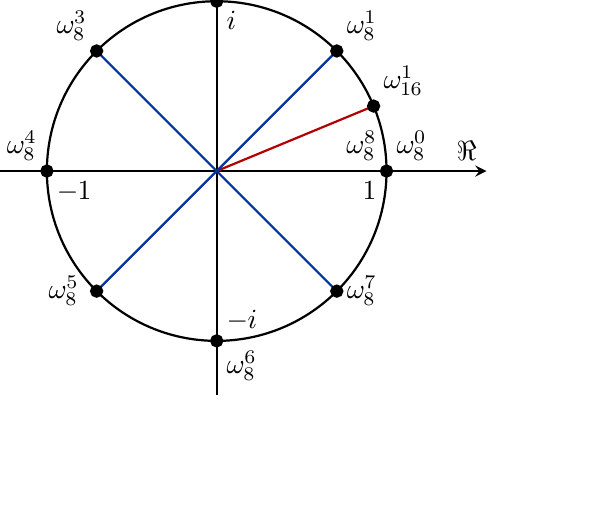
\begin{tikzpicture}
          \begin{axis}[
              axis lines=center,
              axis equal,
              enlargelimits,
              xmin=-1, xmax=1,
              ymin=-1.1, ymax=1.1,
              xlabel={$\Re$},
              ylabel={$\Im$},
              ticks = none,
              thick]
            \draw[radius = 1] (0,0) circle;
            \draw[mark_color] (0,0) -- (0.92387953251,0.38268343236);
            \addplot[black,mark=*] coordinates {(0.92387953251,0.38268343236)} node[above right] {$\omega_{16}^1$};
            \draw[line_color] (0,0) -- (0.70710678118,0.70710678118);
            \draw[line_color] (0,0) -- (-0.70710678118,0.70710678118);
            \draw[line_color] (0,0) -- (-0.70710678118,-0.70710678118);
            \draw[line_color] (0,0) -- (0.70710678118,-0.70710678118);
            \addplot[black,mark=*] coordinates {(1,0)} node[above right] {$\omega_8^0$} node[above left] {$\omega_8^8$} node[below left] {$1$};
            \addplot[black,mark=*] coordinates {(0.70710678118,0.70710678118)} node[above right] {$\omega_8^1$};
            \addplot[black,mark=*] coordinates {(0,1)} node[above right] {$\omega_8^2$} node[below right] {$i$};
            \addplot[black,mark=*] coordinates {(-0.70710678118,0.70710678118)} node[above left] {$\omega_8^3$};
            \addplot[black,mark=*] coordinates {(-1,0)} node[above left] {$\omega_8^4$} node[below right] {$-1$};
            \addplot[black,mark=*] coordinates {(-0.70710678118,-0.70710678118)} node[left,xshift=-0.1cm] {$\omega_8^5$};
            \addplot[black,mark=*] coordinates {(0,-1)} node[below right] {$\omega_8^6$} node[above right] {$-i$};
            \addplot[black,mark=*] coordinates {(0.70710678118,-0.70710678118)} node[right] {$\omega_8^7$};
          \end{axis}
        \end{tikzpicture}
      \end{adjustbox}
    \end{center}
    \caption*{The 8th Roots of Unity and First 16th Root of Unity}
  \end{figure}
}

\newcounter{ButterflyID}
\newcommand\getButterflyID{butterfly\theButterflyID}
\newcommand\genButterflyFilename{\jobname.\getButterflyID.out}

\newcommand{\genButterflyDIF}[2][\genButterflyFilename]{% arg: filename, samples
  \ShellEscape{perl ../common/butterfly-dif.pl #2 > '#1'}%
}

\usetikzlibrary {arrows.meta}

%args: size
\newcommand{\butterfly}[2][\linewidth]{
  \begin{figure}[H]
    \begin{center}
      \begin{tikzpicture}
        \begin{axis}[
            width = #1,
            axis line style={draw=none},
            tick style={draw=none},
            yticklabels={,,},
            xticklabels={,,},
          ] 
          \genButterflyDIF{#2}
          \input{\genButterflyFilename}
        \end{axis}
      \end{tikzpicture}
    \end{center}
    \caption*{The Cooley-Tukey Radix-2 Decimation-In-Frequency Fast Fourier Transform}
  \end{figure}
  \stepcounter{ButterflyID}
}

\usepackage{multicol}
\usepackage{amsmath}

\usepackage[pdfusetitle]{hyperref}

\title{The Fast Fourier Transform}
\author{Zachary Todd Edwards}
\date{\today}

\begin{document}
\maketitle

\section{A Hard Problem}

Lets say we have a wave that we want to find the component frequencies of:

\newcommand{\myWave}[1]{sin(2*2*pi*#1) + sin(3*2*pi*#1)}
\waveform{\myWave{x}}{0}{}

We could try a brute force approach, look at the graphs of sums of sine waves until we get our original:

\waveform{sin(1*2*pi*x) + sin(1*2*pi*x)}{0}{1Hz + 1Hz}
\waveform{sin(1*2*pi*x) + sin(2*2*pi*x)}{0}{1Hz + 2Hz}
\waveform{sin(1*2*pi*x) + sin(3*2*pi*x)}{0}{1Hz + 3Hz}
\waveform{sin(2*2*pi*x) + sin(2*2*pi*x)}{0}{2Hz + 2Hz}
\waveform{sin(2*2*pi*x) + sin(3*2*pi*x)}{0}{2Hz + 3Hz}
%\waveform{sin(3*2*pi*x) + sin(3*2*pi*x)}{0}{3Hz + 3Hz}

We made quite a few assumptions doing this though. We assumed that our wave's amplitude was centered on the horizontal axis and not shifted further up or down, we assumed the phase of our waves is perfect and not shifted left or right, we assumed all of the component frequencies are integers, and we would need to define a range of acceptable error or expect the input wave to be perfect. The first two might also be brute forcible but we are already dealing with a solution too complex to be practical.

Lets try visualizing it in a different way by wrapping our waveform around the origin of a graph:

\begin{multicols}{2}
  \phasor{\myWave{t}}{1}{1}{Rotation Period = 1}
  \phasor{\myWave{t}}{2}{1}{Rotation Period = 2}
  \phasor{\myWave{t}}{3}{1}{Rotation Period = 3}
  \phasor{\myWave{t}}{4}{1}{Rotation Period = 4}
\end{multicols}

The dot is the center or average of this wound up version of our waveform, and we can see that it is almost always very close to zero except when the rotation period is 3 or 2, which is also the component frequencies of our wave!

\pagebreak

\section{Euler's Formula}
Okay thats great but what is the actual math behind this? Wrapping the function around the origin is not any simpler visually than brute forcing, and even though we only had to check each frequency once getting that average is an extra step. Also, what is rotation period and how do we change it? The axis labels have already given away part of the secret, these wrappings are being graphed on the complex plane!

If you have spent any amount of time studying math you have likely ran into the so-called most beautiful equation in mathematics: $e^{i\pi}+1=0$. This is Euler's identity and its big cousin Euler's formula is the secret to this winding. How does it work though?  Why does $e^{i\pi}+1$ equal zero?

\unitCircle

The very short version is that it is a simplification of the full formula which is $e^{i\theta}=cos(\theta)+i\cdot sin(\theta)$. It is also worth noting that this is continuous and works for angles larger than $2\pi$ or less than 0.

\pagebreak

\section{Spiralling a Function}

If Euler's formula always has a distance from the origin of 1 rotated by $\theta$ radians and multiplying anything by 1 is itself, could we just plug in our variable times $2\pi$ for $\theta$ and then multiply our function with that to wrap it around the origin? This is math, there is no way it could be that easy, could it?

\begin{multicols}{2}
  \polynomial{x}{$F(x)=x$}
  \phasor{t}{1}{0}{$F(x)\cdot e^{ix2\pi}$ where $x \ge 0$}
\end{multicols}

It really is that easy! Above is a spiraled version of the equation $F(x) = x$, for positive x so it is more readable, we can see by looking at the positive real axis that for every one full rotation it increases by one unit of distance from the origin. This can be seen in all of the axes, with the other ones having quarter, half, and three-quarter offsets from the last integer.

What about rotational period, what does that even mean? That is how many full rotations we do for one unit increase to the input of our original function, and how we can do this is already sneakily built in to the original formula, for a period of one we multiply $2\pi$ by one, for a period of two we multiply it by two, etc. If we omit $2\pi$ we get a rotation period of $\frac{1}{2\pi}$, we can think of it as dividing $2\pi$ by itself.

\begin{multicols}{2}
  \phasor{t}{2}{0}{$F(x)\cdot e^{ix2\cdot 2\pi}$ where $x \ge 0$}
  \phasor{t}{3}{0}{$F(x)\cdot e^{ix3\cdot 2\pi}$ where $x \ge 0$}
\end{multicols}

\pagebreak

\section{The Continuous Fourier Transform}

There is one last piece needed to get our winding solution to work: the average. Conveniently for us we have a quick way of getting the total area under a curve, we can take its integral and divide by the total time the wave occupies:

\begin{displaymath}
  \hat{G}(f) = \frac{1}{N}\int_{0}^{N} G(x) \cdot e^{2\pi ifx}dx
\end{displaymath}

This works! When graphed we will get something like this:

\fourierSpectrum[0.7\linewidth]{4}{6}{512}{\myWave{x}}{$\hat{G}(f)$ for $G(x) = sin(2 \cdot 2\pi x) + sin(3 \cdot 2\pi x)$}

This is not quite the true Fourier transform though, there are a few adjustments to get there. The true Fourier transform does not take the average, just the total. With the average it is sometimes called the ``normalized Fourier transform.'' The Fourier transform also does not typically specify a time frame, and instead goes from $-\infty$ to $+\infty$, assuming that the wave itself needs to start and stop somewhere. The winding is also usually done in the clockwise direction, so the exponent is negated. Finally, the variable being integrated is usually $t$. With all this:

\begin{displaymath}
  \hat{G}(f) = \int_{-\infty}^{\infty} G(t) \cdot e^{-2\pi ift}dt
\end{displaymath}

There is just one problem: computers tend to not like continuity or infinity.

\pagebreak

\section{The Discrete Fourier Transform}

Well if computers do not handle continuous functions very well then how will we get the input waveform in the first place, let alone process it? The answer might seem obvious, just take discrete points, also called samples, on the waveform at regular intervals and perform the Fourier transform on them. Lets try it, we will take a high number of samples from our original wave, wrap them around the origin, and sum up their results when multiplied with $e^{i\theta}$ at regular intervals.

\waveform{\myWave{x}}{32}{32 samples across 4 seconds, for a sample rate of 8 per second.}

\begin{multicols}{2}
  \phasor{\myWave{t}}{3}{32}{Rotation Period = 3}
  \phasor{\myWave{t}}{4}{32}{Rotation Period = 4}
\end{multicols}
{\begin{multicols}{2}
  \raggedcolumns
  The discrete version of the Fourier transform should be relatively easy to reverse engineer:
  \begin{displaymath}
    X_k = \sum_{n=0}^{N-1} x_n \cdot e^{-\frac{i2\pi}{N}kn}
  \end{displaymath}
  It is convention to use $x_n$ for the input set and $X_n$ for the output set, both of size $N$. We might also want to normalize the output:
  \begin{displaymath}
    X_k = \frac{1}{N} \sum_{n=0}^{N-1} x_n \cdot e^{-{\frac{i2\pi}{N}kn}}
  \end{displaymath}
  With all that we get the following for our graph:

  \fourierSpectrum{4}{8}{32}{\myWave{x}}{}
\end{multicols}}

This doesn't look right, there are peaks at 2hz and 3hz but also 5hz and 6hz, and it looks symmetrical. What is going on?

\pagebreak

\section{Nyquist-Shannon}

Our graph of the discrete Fourier transform above is actually correct, but the oddness in its results hints at a deeper problem we are bumping up against: how do we know how many points are enough?

\criticalFrequency{}

All of these waveforms have the same samples at the same sample rate. The problem is not just that these different waves produce the same samples in this one case, its that these samples have many different waves that could fit them. It gets worse, there are infinitely many waveforms that could fit any set of discrete points, we need to know some constraints on the waveform coming in in order to do anything useful with the samples.

The symmetry of our spectrum graphs above actually give us a hint about it, here is one with double the sample rate:
\fourierSpectrum[0.5\linewidth]{4}{16}{64}{\myWave{x}}{}
The results got more accurate, as expected, but the center of symmetry doubled as well. This ``center of symmetry'' is called the Nyquist limit, and is the highest frequency that discrete samples can represent without a loss in fidelity. Conveniently the Nyquist limit is just half of our sample rate, non-inclusive. The symmetrical second half is the complex-conjugate of the first half, and is usually ignored when working with real-numbered inputs.

Which frequency a particular index corresponds to, its frequency bin, can be gotten with $k\frac{f_s}{N}$
where $k$ is the index of the result, $f_s$ is the sample rate per-second, and $N$ is the total number of samples. The magnitude, absolute value, of each entry is usually what is graphed in charts like the ones above. The imaginary part of each entry tells us that frequency's phase, how much it is shifted left or right.
\pagebreak

\section{Complex Programming}

Before we can start translating this math into code there is one last hurdle: how do we write programs with complex numbers? The good news is that most programming languages include complex numbers as part of their standard library, or as part of a common third party library.

C does some macro magic to ``overload'' the operators for complex types, but cannot overload the functions so there is a separate set of math functions for them, as well as a few macros for assignment:
\begin{lstlisting}
  #include <complex.h>
  void dft(double complex *x, double complex *X, int N){
    for(int i = 0; i < N; i++)
      X[i] = CMPLX(0.0, 0.0);

    for(int k = 0; k < N; k++)
      for(int n = 0; n < N; n++)
        X[k] += x[n] * cexp(-(((I * 2 * M_PI) / N) * k * n));
  }
\end{lstlisting}

C++ is similar but uses templates:
\begin{lstlisting}
  #include <vector>
  #include <complex>
  void dft(std::vector<std::complex<double>> &x, 
           std::vector<std::complex<double>> &X, int N){
    X.clear();
    X.resize(N, 0);

    for(int k = 0; k < N; k++)
      for(int n = 0; n < N; n++)
        X[k] += x[n] * std::exp(-(((1.0i * 2 * M_PI) / N) * k * n));
  }
\end{lstlisting}

Perl:
\begin{lstlisting}[language=Perl]
  use Math::Complex;
  sub DFT{
    my ($x, $X) = @_;
    my $N = scalar(@$x);
    @$X = ();

    for(my $k = 0; $k < $N; $k++){
      for(my $n = 0; $n < $N; $n++){
        $$X[$k] += $$x[$n] * exp(-(((i * 2 * pi) / $N) * $k * $n));
      }
    }
  }
\end{lstlisting}

The complexity of this algorithm is $O(N^2)$, however, and we are going to want to be able to process frequencies in the gigahertz range. To make this practical we need to somehow speed this up.

\pagebreak

\section{A Simpler Problem}
Lets tackle a similar but simpler problem, how can we get a set of points on a polynomial?

Say we have a class for our points that looks like:
\begin{lstlisting}
  class point{
    double x, y;
    point(_x, _y) : x(_x), y(_y){}
  };
\end{lstlisting}

Next our function prototype looks like:
\begin{lstlisting}
  vector<point> polynomial(int degree, double coefficients[], int n);
\end{lstlisting}

We might try to use the brute force method:
\begin{lstlisting}
  vector<double> points(n);
  for(int x = 0; x < n; x++){
    double y = coefficients[0];
    for(int j = 1; j <= degree; j++){
      y += coefficients[j] * pow(x,j);
    }
    points[x] = point(x,y);
  }
  return samples;
\end{lstlisting}
However, this takes $O(nk)$ time where n is the degree of the polynomial and k is the number of samples needed, this is also not counting the not-insignificant time pow() can take. Is there a faster way?

\section{Symmetry}
Lets look at a few graphs of polynomials:

\begin{multicols}{2}

  \polynomial{2*x}{$F(x)=2x$}
  \polynomial{1/2*x^2}{$F(x)=\frac{1}{2} x^2$}
  \polynomial{x^2+x^3}{$F(x)=x^2+x^3$}
  \polynomial{3*x^3-x^4}{$F(x)=3x^3-x^4$}
  \polynomial{x+(1/3)*x^3}{$F(x)=x+\frac{1}{3}x^3$}
  \polynomial{x^4+1}{$F(x)=1+x^4$}

\end{multicols}

Some of these are symmetrical across the vertical axis, some of them are symmetrical across both axes, and some of them look almost symmetrical but aren't quite. What is the difference in the polynomials that are symmetrical and those that aren't?

The polynomials with only even-powered terms or odd-powered terms are symmetrical, with the former being across the vertical axis: $F(x) = F(-x)$, and the latter being symmetrical across both: $F(x) = -F(-x)$. Most polynomials don't only contain terms of the same parity, so how can we take advantage of this?

\pagebreak

\section{Polynomial Decomposition}

Lets take the following rather wooly polynomial:

\polynomial[0.6\textwidth]{x-3*x^2+2*x^3+4*x^4+x^5-1}{$F(x)=-1x-3x^2+2x^3+4x^4+x^5$}

Lets try separating it into its odd and even terms:

\begin{multicols}{2}
  \polynomial{-1-3*x^2+4*x^4}{$F_e(x)=-1-3x^2+4x^4$}
  \polynomial{x+2*x^3+x^5}{$F_o(x)=x+2x^3+x^5$}
\end{multicols}

These are both symmetrical and when added together we get our original polynomial, we might be able to work with this.

\pagebreak

Lets try writing another algorithm to take advantage of this, to try to keep it as simple as possible we will assert that n, the number of points we want, is even:

\begin{lstlisting}
  vector<point> points;
  assert(!(n % 2));
  for(int x = 1; x <= n / 2; x++){
    double yp = coefficients[0];
    double yn = coefficients[0];
    for(int j = 1; j <= degree; j++){
      double term = pow(x,j);
      yp += term;
      yn += (j % 2) ? -term : term;
    }
    points.push_back(point(x,yp));
    points.push_back(point(-x,yn));
  }
  return points;
\end{lstlisting}

Gross! Not only is this inelegant, it does not save us that much time either; asymptotically it is the same. Lets go back to our polynomials and see what more we can squeeze out of them.

We can factor an $x$ out of the odd terms so that we get $F_o(x)=x(1+2x^2+x^4)$ or $x F_o(x)=1+2x^2+x^4$. Putting this together we get $F(x) = F_e(x) + xF_o(x)$ and now that $F_o(x)$ is all even terms it would be the same for positive and negative inputs. This could possibly eliminate the ternary operator above which might benefit performance a bit, but we are still stuck with the same complexity. To get any noticeable benefit we need a way to do this recursively.

We can start by trying to make $F_e(x)$ and $F_o(x)$ polynomials with their own odd and even terms. All of the terms in each of these are even, so we could divide the exponents by two and square the inputs. This gives us $F_e(x)=-1-3x+4x^2$ and $F_o(x)=1+2x+x^2$ resulting in our original polynomial being $F(x) = F_e(x^2) + x F_o(x^2)$.

We have a new problem now though; if we try to recursively apply this method our input is always positive or zero after the first decomposition because it was squared, so the variable we factor out of the odd term polynomial will always be positive, and the whole point of separating out the odd and even terms in the first place was that they behaved differently with negative inputs. There is also the problem of magnitude, this repeated squaring of the inputs actually breaks the equivalence if we try to apply it more than once. We have two inputs that cooperate with this method, 0 and 1, since they are already positive and their squares have the same magnitude, what we need are more ones. We used the complex exponential $e^{ix}$ as a kind of ``1'' before, would it work here?
\pagebreak

\section{The Roots of Unity}

\rootsOfUnity

For real numbers, $\sqrt{1}$ has two answers, 1 and -1, and this is true for complex numbers as well. Higher roots get more interesting, for real numbers $\sqrt[3]{1}$ has only one answer which is 1, however for complex numbers $\sqrt[3]{1}$ has three answers: 1, $e^\frac{i2\pi}{3}$, $e^\frac{i4\pi}{3}$. Higher roots have more complex results; the n-th root of 1 has n complex values and these are the roots of unity. The first root of unity after 1 is generally denoted with $\omega$ (omega), and the j-th root of unity for the n-th complex root of 1 would be $\omega_n^j$.

The roots of unity have a few useful properties: they always add up to zero, their absolute value is always one, all equivalent ratios of $j$ and $n$ for $\omega_n^j$ are equivalent eg $\omega_8^2 = \omega_4^1$, negation ``flips'' their position eg $-\omega_8^1 = \omega_8^5$, and they are cyclical when raised to a power or multiplied eg ${\omega_8^3}^{10} = \omega_8^3 \cdot \omega_8^{10} = \omega_8^{30} = \omega_8^6$. Since getting the square root of a complex number is relatively trivial these properties lets us quickly get power-of-two-first-roots of unity by repeatedly getting the square root (raising to the power of $\frac{1}{2}$) of $\omega$.

The roots of unity can also be calculated using $e^\frac{i2\pi j}{n}$, this is equivalent to the exponential used in the discrete transform.

\pagebreak

Complex numbers can be written as $a + bi$, with this the formula for getting the square root of a complex number is:
\begin{displaymath}
  \sqrt{a+ib} = \pm\left(\sqrt{\frac{|z| + a}{2}} + i\sqrt{\frac{|z| - a}{2}}\right) \text{ when } b \ge 0
\end{displaymath}
\begin{displaymath}
  \sqrt{a+ib} = \pm\left(\sqrt{\frac{|z| + a}{2}} - i\sqrt{\frac{|z| - a}{2}}\right) \text{ when } b < 0
\end{displaymath}

The absolute value of a complex number is $\sqrt{a^2+b^2}$ and squaring a complex number is the same as real algebra, keeping an eye our for anytime an $i$ gets squared to replace it with -1. If we are only dealing with $a + bi$ we can treat it like a binomial and the squaring formula is $a^2 - b^2 + 2abi$. Lets run through a few examples to see all of this in action:
\begin{multicols}{2}
  \null \vfill
  \begin{align*}
    \sqrt{i} = \sqrt{0+1i} & = \sqrt{\frac{|0+1i| + 0}{2}} + i\sqrt{\frac{|0+1i| - 0}{2}} \\
                           & = \sqrt{\frac{1}{2}} + i\sqrt{\frac{1}{2}}                   \\
                           & = \frac{1}{\sqrt{2}} + \frac{i}{\sqrt{2}}                    \\
                           & = \frac{1+i}{\sqrt{2}}
  \end{align*}
  \vfill \null
  \columnbreak
  \null \vfill
  \begin{align*}
    \left(\frac{1+i}{\sqrt{2}}\right)^2 & = \frac{1+i}{\sqrt{2}} \cdot \frac{1+i}{\sqrt{2}} \\
                                        & = \frac{(1+i)(1+i)}{\sqrt{2}\cdot\sqrt{2}}        \\
                                        & = \frac{1+2i+i^2}{2}                              \\
                                        & = \frac{1+2i-1}{2}                                \\
                                        & = \frac{2i}{2}                                    \\
                                        & = i
  \end{align*}
  \vfill \null
\end{multicols}

C and C++ complex square roots handle multiple possible results by making a ``branch cut along the negative real axis.'' If we visualize the square root rotating a number around the complex plane, if it has multiple results it will favor the one that does not cross the negative real axis. Putting all of this together we can generate a list of first roots-of-unity like this:
\begin{lstlisting}
std::vector<std::complex<double>> gen_omegas(long N, bool inverse) {
  int Nth = (bit_length(N) - 1); // log_2(N)
  std::vector<std::complex<double>> omegas;
  omegas.push_back(-1 + 0i);
  omegas.push_back(0  - 1i);
  for (int j = 2; j < Nth; j++) omegas.push_back(std::sqrt(omegas[j - 1]));
  if (inverse)
    for (int j = 1; j < Nth; j++) omegas[j] = std::conj(omegas[j]);
  return omegas;
}
\end{lstlisting}

\texttt{bit\_length(x)} is the number of bits required to represent a number and that is the integer $log_2(x) + 1$. This is much faster than using the floating-point log functions, most modern CPUs can do this in a single instruction. We can implement this in C++20, otherwise compiler intrinsics need to be used:
\begin{lstlisting}
#include <bits>
#include <climits>
int bit_length(unsigned long){
  return (CHAR_BIT * sizeof N) - std::countl_zero(x);
}
\end{lstlisting}

\pagebreak

\section{The Fast Fourier Transform}
Putting all of this together:
\begin{center}
  \begin{tabular}{llll}
    $F(x)$      & \multicolumn{2}{l}{$= -1+x-3x^2+2x^3+4x^4+x^5$} & $=F_e(x^2)+xF_o(x^2)$                                \\
    $F_e(x)$    & $=-1-3x+4x^2$                                   &                       & $=F_{ee}(x^2)+xF_{eo}(x^2)$  \\
    $F_o(x)$    & $=1+2x+x^2$                                     &                       & $= F_{oe}(x^2)+xF_{oo}(x^2)$ \\
    $F_{ee}(x)$ & $=-1+4x$                                        & $F_{eo}(x)=-3$        &                              \\
    $F_{oe}(x)$ & $=1+x$                                          & $F_{oo}(x)=2$         &                              \\
  \end{tabular}
\end{center}

Plugging in our roots of unity:
\begin{center}
  \begin{tabular}{ll | ll | ll}
    $F_{ee}(1)$  & $= 3$  & $F_e(1)$  & $= 0$       & $F(1)$         & $= 4$                    \\
    $F_{ee}(-1)$ & $= -5$ & $F_e(i)$  & $= 5 - 3i$  & $F(\omega)$    & $= - 5 - 3i + 2\omega i$ \\
    $F_{eo}(1)$  & $= -3$ & $F_e(-1)$ & $= 6$       & $F(i)$         & $= 6$                    \\
    $F_{eo}(-1)$ & $= -3$ & $F_e(-i)$ & $= -5 + 3i$ & $F(\omega i)$  & $= - 5 + 3i + 2\omega$   \\
    $F_{oe}(1)$  & $= 1$  & $F_o(1)$  & $= 2 + 2$   & $F(-1)$        & $= -4$                   \\
    $F_{oe}(-1)$ & $= 0$  & $F_o(i)$  & $= 2i$      & $F(-\omega)$   & $= - 5 - 3i - 2\omega i$ \\
    $F_{oo}(1)$  & $= 2$  & $F_o(-1)$ & $= 0$       & $F(-i)$        & $= 6$                    \\
    $F_{oo}(-1)$ & $= 2$  & $F_o(-i)$ & $= -2i$     & $F(-\omega i)$ & $= - 5 + 3i - 2\omega$   \\
  \end{tabular}
\end{center}

Lets compare these answers to the results of the discrete Fourier transform for the same input set, we can pad in input set with 0s to get the discrete Fourier transform to output the same number of values, these are equivalent to coefficients of 0 for higher degree terms so it does not effect the value of the polynomial. We effectively were already doing this above.
\begin{center}
  \begin{tabular}{ |c|c|c|c|c|c|c|c|c| }
    \hline
    Input  & -1 & 1           & -3 & 2           & 4  & 1           & 0 & 0           \\
    \hline
    Output & 4  & -6.41-1.59i & 6  & -3.59+4.41i & -4 & -3.59-4.41i & 6 & -6.41+1.59i \\
    \hline
  \end{tabular}
\end{center}

It is a perfect match, and with $O(NlogN)$ complexity! Lets write some code to calculate this, since the FFT can be calculated in-place X will be used as the input and overwritten:
\begin{lstlisting}
  void fft(std::vector<std::complex<double>> omegas, 
           std::vector<std::complex<double>> &X, long N) {
    assert((N & (N - 1)) == 0);
    for (long n = 2; n <= N; n *= 2) {
      std::complex<double> omega = omegas[bit_length(n) - 2];
      std::complex<double> root_of_unity = 1;
      for (long j = 0; j < n / 2; j++) {
        for (long k = 0; k < N; k += n) {
          std::complex<double> product = root_of_unity * X[k + j + n / 2];
          X[k + j + n / 2] = X[k + j] - product;
          X[k + j] = X[k + j] + product;
        }
        root_of_unity *= omega;
      }
    }
  }
\end{lstlisting}

Lets run it and see what it does:

\begin{center}
  \begin{tabular}{ |c|c|c|c|c|c|c|c|c| }
    \hline
    Input  & -1 & 1        & -3       & 2         & 4  & 1         & 0        & 0        \\
    \hline
    Output & 4  & 0.1-2.9i & 1.0+5.0i & -4.1+7.1i & -6 & -4.1-7.1i & 1.0-5.0i & 0.1+2.9i \\
    \hline
  \end{tabular}
\end{center}

This is not correct! This code is actually good, there is just one more thing we are missing.

\pagebreak

\butterfly{8}

If we actually draw out how values are reused we get something like the above, usually called a butterfly diagram. Each of the sets of arrows are sometimes called a ``butterfly operation.'' The part we are missing is the input ordering, we need to get the inputs in their order after the recursive even/odd separating. Alternatively we could do the operations backwards, start with the inputs in-order and do the size $N$ butterfly operation then the size $\frac{N}{2}$ butterfly operation and so on, but then the output would be in this peculiar ordering anyway and we would have to get the first 8th root of unity from the start instead of being able to take the square root each pass. This ordering is actually a little insidious, take a second to see if you can figure out a non-recursive way to describe the ordering.

The ordering is called bit-reversal-permutation, the index of each element in this ordering is the bits of the original index reversed. With the input in this order we, at last, get:
\begin{center}
  \begin{tabular}{ |c|c|c|c|c|c|c|c|c| }
    \hline
    Input  & -1 & 1           & -3 & 2           & 4  & 1           & 0 & 0           \\
    \hline
    Output & 4  & -6.41-1.59i & 6  & -3.59+4.41i & -4 & -3.59-4.41i & 6 & -6.41+1.59i \\
    \hline
  \end{tabular}
\end{center}

\end{document}